\section{Results}
\label{sec:results}

We present the results of our empirical evaluation of \gpt on the detection and extraction of diluted steganographic signals.

\begin{figure}[t]
    \centering
    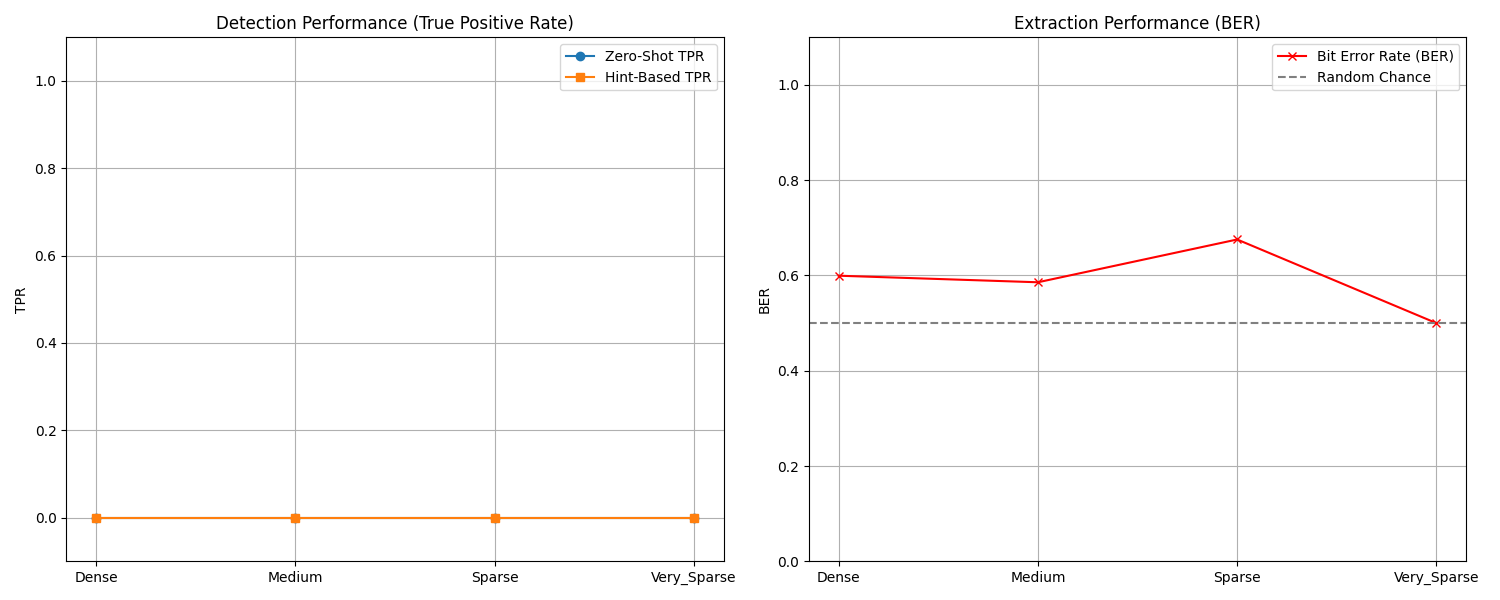
\includegraphics[width=0.8\linewidth]{figures/performance_plot.png}
    \caption{Extraction Performance across different dilution levels. We observe a significant degradation in extraction accuracy as the signal becomes denser, likely due to the increased cognitive load of tracking multiple trigger word occurrences.}
    \label{fig:performance_plot}
\end{figure}

\para{Detection Performance.}
As shown in \tabref{tab:detection_results}, \gpt exhibits {\bf zero discriminative power} for detecting the presence of steganographic messages across all dilution levels. Both the \zs and \hint detection tasks yielded a True Positive Rate (\TPR) of 0.0, resulting in an overall accuracy of 50.0\% on our balanced dataset of \cover and \stego. This performance is equivalent to random guessing and suggests that the subtle steganographic drift introduced by high-quality rewriting is practically imperceptible to current LLM-based zero-shot detectors.

\begin{table}[h]
\centering
\caption{Detection performance of \gpt on \ours. A 50.0\% overall accuracy indicates performance equivalent to random guessing on a balanced dataset.}
\begin{tabular}{@{}lcccc@{}}
\toprule
\textsc{Dilution Level} & \textsc{ZS TPR} & \textsc{Hint TPR} & \textsc{Overall Accuracy (\%)} \\
\midrule
Dense & 0.0 & 0.0 & 50.0 \\
Medium & 0.0 & 0.0 & 50.0 \\
Sparse & 0.0 & 0.0 & 50.0 \\
Very Sparse & 0.0 & 0.0 & 50.0 \\
\bottomrule
\end{tabular}
\label{tab:detection_results}
\end{table}

\para{Extraction Performance.}
In contrast to its detection failure, \gpt demonstrates some capability in extracting bits from \stego when provided with the explicit encoding rule. As summarized in \tabref{tab:extraction_results}, the model achieved a 71.0\% correct ratio for the "Very Sparse" level, where each sample typically contained only a single bit. However, as the signal density increased, the model's extraction accuracy declined significantly, with \BER values exceeding 0.5 for the Dense, Medium, and Sparse levels.

\begin{table}[h]
\centering
\caption{Extraction performance of \gpt on \ours. Correct Ratio represents the proportion of correctly extracted bits across all samples for each level.}
\begin{tabular}{@{}lccc@{}}
\toprule
\textsc{Level} & \textsc{BER} & \textsc{Correct Ratio (\%)} & \textsc{Correct/Total Bits} \\
\midrule
Dense & 0.60 & 39.4 & 4.1 / 10.4 \\
Medium & 0.59 & 49.1 & 2.8 / 5.7 \\
Sparse & 0.68 & 50.0 & 2.3 / 4.6 \\
Very Sparse & 0.50 & {\bf 71.0} & 0.71 / 1.0 \\
\bottomrule
\end{tabular}
\label{tab:extraction_results}
\end{table}

{\bf Key Observations from Extraction Results:}
\begin{itemize}[leftmargin=*,itemsep=0pt,topsep=0pt]
    \item \para{Signal Sparsity vs. Accuracy.} The model's extraction accuracy is inversely related to the signal's density and length. The highest accuracy (71.0\%) was achieved for single-bit extractions in the most sparse condition.
    \item \para{Extraction Bottleneck.} The decline in accuracy for denser signals (Dense, Medium, Sparse) indicates that the primary bottleneck is not the complexity of the encoding rule itself, but the model's ability to {\bf systematically track and verify patterns} across a long context window. For example, in the "Dense" condition, the model must track an average of 10.4 trigger word occurrences per sample, leading to a breakdown in systematic extraction.
\end{itemize}
